\section{Résultats}

\subsection{Mortalité routière}

\subsubsection{Observation de carcasses}





\subsubsection{Persistance de carcasses sur la route}


\subsubsection{Observations complémentaires}



\subsection{Suivi de la petite faune}

\subsubsection{Pièges photographiques}
Un total de \mbox{2 584 774} images prises en 2025 sur les trente ponceaux à l'étude ont été traitées par MegaDetector, nécessitant \mbox{5 780 601} secondes de temps de calcul, équivalant à 66.9 jours de calcul en continu. À partir de ces images traitées, nous avons terminé la validation des images de 18 ponceaux, ce qui représente 54\% des photos du jeu de données. Nous avons inspecté les 38 110 images étiquetées par MegaDetector comme ayant des détections animales pour lesquelles la confiance était $\geq 75$\% dans ces 18 ponceaux. La validation de ces images par un humain a révélé que le taux de vrais positifs était de 45.95\%: 19 090 des détections étaient de vraies détection d'animaux. Le taux de faux positifs était de 54.05\% (i.e., détections présumées par MegaDetector mais non avérées). À partir des 38 110 images étiquetées par MegaDetector, nous avons également noté des faux-négatifs, c'est-à-dire, des sections d'images où MegaDetector n'avait pas déclaré la présence d'un animal. À partir de l'inspection des images des 18 ponceaux pour lesquelles le seuil de confiance $\geq 75$\%, nous avons détecté 2 465 animaux additionnels. Un total de 39 121 détections animales ont été répertoriées sur les 1 395 515 images des 18 ponceaux.

Différents groupes et espèces ont été observées sur les images, incluant des invertebrés (araignées, odonates, papillons) et plusieurs vertébrés (Tableau \ref{tab:cam-sp}). Des 39 121 détections animales, 78\% étaient des mammifères de moyenne taille et 13\% étaient de la sauvagine. Les autres animaux détectés étaient des oiseaux forestiers (7\%), des petits mammifères (1\%), des reptiles (0.2\%) et des amphibiens (0.6\%) (Fig. \ref{fig:cam-Prop}. La répartition actuelles des observations selon les types de tronçons ne suggère pas de patrons particuliers pour le moment, mis à part les petits mammifères qui semblaient plus fréquents dans les tronçons de catégorie 2 (milieu humide de chaque côté), bien qu'il reste environ 50\% des images à valider (Fig. \ref{fig:cam-Prop-Type}).

\begin{table}
  \caption{Espèces et groupes d'espèces répertoriées sur les images prises par les pièges photographiques dans les ponceaux des tronçons suivis en 2025. Le tableau a été préparé à partir des 39 121 détections animales provenant des 18 tronçons analysés.}
  \label{tab:cam-sp}
  \begin{tabular}{p{0.3\textwidth}p{0.7\textwidth}}
    \hline
    Groupe & Espèces ou niveau taxonomique supérieur \\
    \hline
    Amphibiens & Anoures (\emph{Lithobates} sp.) \\
    Reptiles & Couleuvres et tortues (\emph{Chelydra serpentina}) \\
    Oiseaux forestiers & Passereaux et dindon sauvage (\emph{Meleagris gallopavo}) \\
    Sauvagine & Canards, bernaches (\emph{Branta canadensis}) et échassiers (grand héron \emph{Ardea herodias}, héron vert \emph{Butorides virescens}, bihoreau gris \emph{Nycticorax nycticorax}) \\
    Petits mammifères & Écureuil roux (\emph{Tamiasciurus hudsonicus}), écureuil gris (\emph{Sciurus carolinensis}), musaraigne (\emph{Sorex} sp.), polatouche (\emph{Glaucomys} sp.), souris (\emph{Zapus hudsonius} ou \emph{Napaeozapus insignis}), campagnols (\emph{Microtus pennsylvanicus} ou \emph{Clethrionomys gapperi}), tamia rayé (\emph{Tamias striatus}) \\
    Mammmifères moyens & castor du Canada (\emph{Castor canadensis}), chat domestique (\emph{Felis catus}), chien domestique (\emph{Canis familiaris}), lièvre d’Amérique (\emph{Lepus americanus}), loutre de rivière (\emph{Lontra canadensis}), marmotte commune (\emph{Marmota monax}),  mouffette rayée (\emph{Mephitis mephitis}), \emph{Mustela} sp., opossum de Virginie (\emph{Didelphis virginiana}), rat surmulot (\emph{Rattus norvegicus}), raton laveur (\emph{Procyon lotor}, rat musqué (\emph{Ondatra zibethicus}), renard roux (\emph{Vulpes vulpes}), vison d'Amérique (\emph{Vison vison}) \\
    Grands mammifères & Cerf de Virginie (\emph{Odocoileus virginianus}) \\
    Invertébrés & Araignées, lépidoptères et odonates \\
   \hline
  \end{tabular}
\end{table}


\begin{figure}
  \centering
  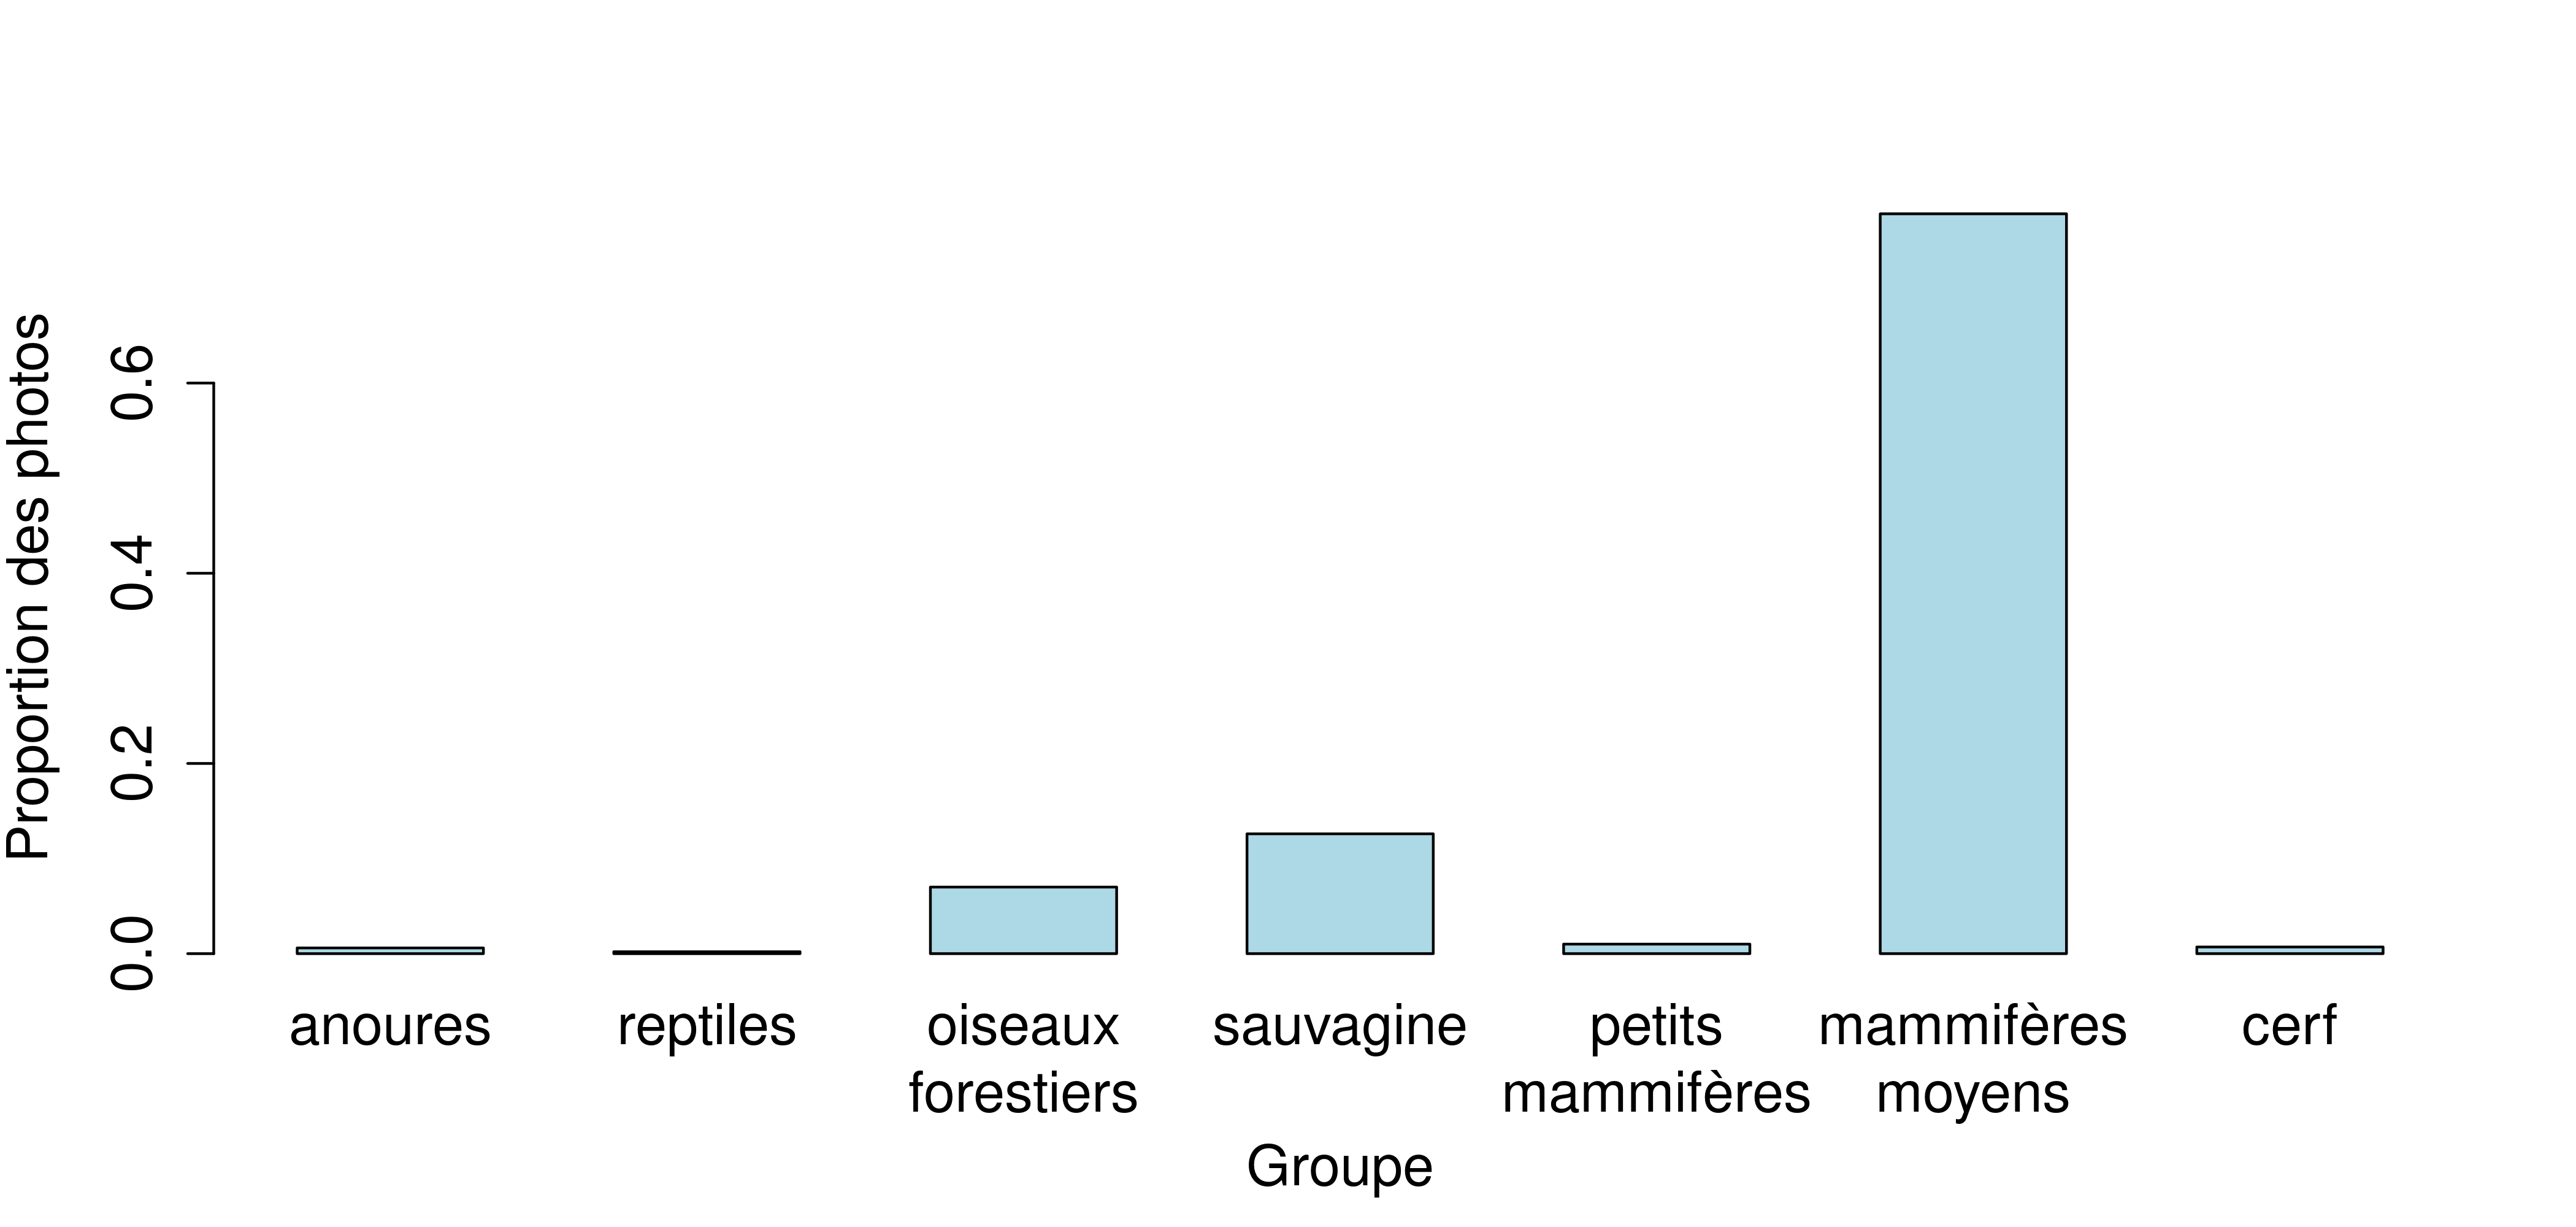
\includegraphics[width=0.9\textwidth]{fig/cam-Prop.png}
\caption{Proportions des images avec détection animales de vertébrés prises par les pièges photographiques dans les ponceaux des tronçons suivis en 2025. La figure a été préparée à partir des 39 121 détections animales provenant des 18 tronçons analysés.}
\label{fig:cam-Prop}
\end{figure}


\begin{figure}
  \centering
  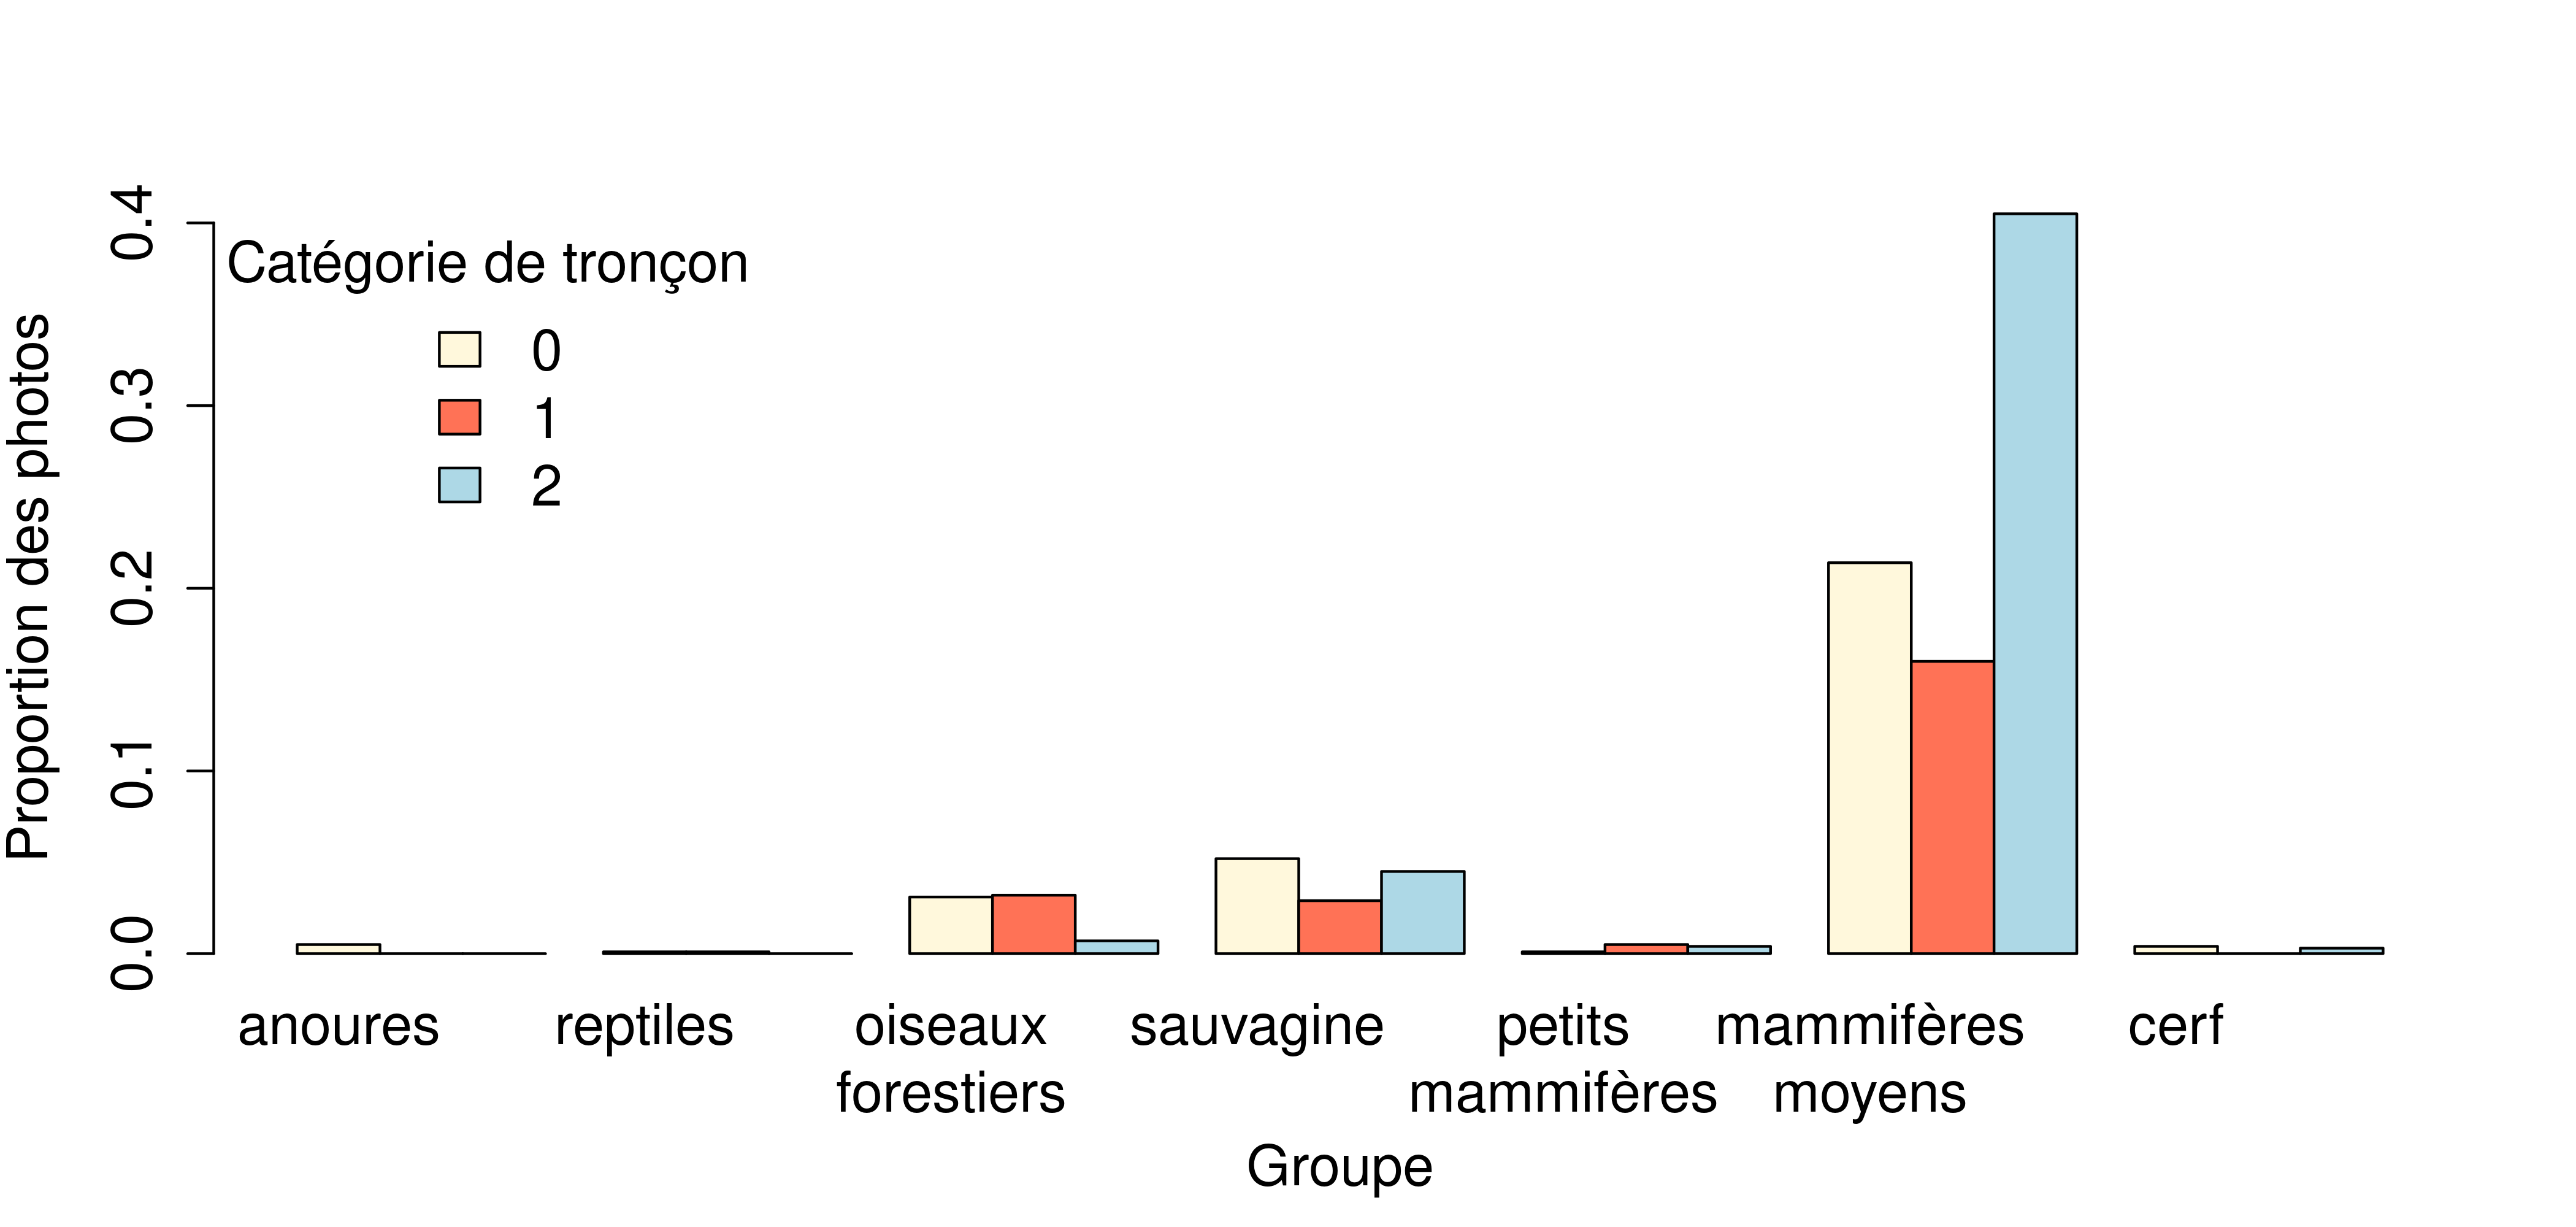
\includegraphics[width=0.9\textwidth]{fig/cam-Prop-Type.png}
\caption{Proportions des images avec détection animales de vertébrés prises par les pièges photographiques dans les ponceaux des tronçons suivis en 2025 selon les trois différentes types de tronçons échantillonnés. La figure a été préparée à partir des 39 121 détections animales provenant des 18 tronçons analysés.}
\label{fig:cam-Prop-Type}
\end{figure}






\subsubsection{Enregistrements acoustiques}



\subsubsection{Recherche par drones}





\subsubsection{Stations de plaques à reptiles}
